\NeedsTeXFormat{LaTeX2e}
%\PassOptionsToClass{handout}{beamer}
\documentclass{beamer}
\usepackage{beamerPack}
\usepackage[boxed,ruled,vlined]{algorithm2e}
\usepackage[05]{../lecture}
\usepackage[usestackEOL]{stackengine}[2013-10-15]
\def\x{\hspace{4.1ex}}    %BETWEEN TWO 1-DIGIT NUMBERS
\def\y{\hspace{3.4ex}}  %BETWEEN 1 AND 2 DIGIT NUMBERS
\def\z{\hspace{2.7ex}}    %BETWEEN TWO 2-DIGIT NUMBERS
\subtitle{}
\begin{document}

\begin{frame}[fragile]{}
\titlepage
\end{frame}

\section{algorithm design}		%%%%%%%%
\subsection{}

\begin{frame}[fragile]{帰納法とループ}{与えられた数式からプログラムへ}
\begin{align*}
Fib(0) =& 1\\
Fib(1) =& 1\\
Fib(n) =& Fib(n - 1) + Fib(n - 2)\\
\end{align*}

\begin{align*}
A(0, n) =& n + 1\\
A(m + 1, 0) =& A(m, 1)\\
A(m + 1, n + 1) =& A(m, A(m + 1, n))
\end{align*}
\end{frame}

\begin{frame}[fragile]{再帰とループ}{与えられた問題からプログラムへ}
\stackMath
\Longstack[l]{
n=0\\
n=1\\
n=2\\
n=3\\
n=4\\
n=5\\
n=6\qquad\ \\
}
\Longstack{
1\\
1\x 1\\
1\x 2\x 1\\
1\x 3\x 3\x 1\\
1\x 4\x 6\x 4\x 1\\
1\x 5\y 10\z 10\y 5\x 1\\
1\x 6\y 15\z 20\z 15\y 6\x 1\\
1\x 7\x 21\z 35\z 35\z 21\y 7\x 1\\
}

$n = 23$, 左から11番目の数は?
\end{frame}


\begin{frame}[fragile]{Pascalの三角形}{北東+北西に等しい}

\begin{align*}
P(n,k) &= P(n-1, k - 1) + P(n - 1, k)
\end{align*}

\begin{center}
\rotatebox{-45}{
\scalebox{0.6}{
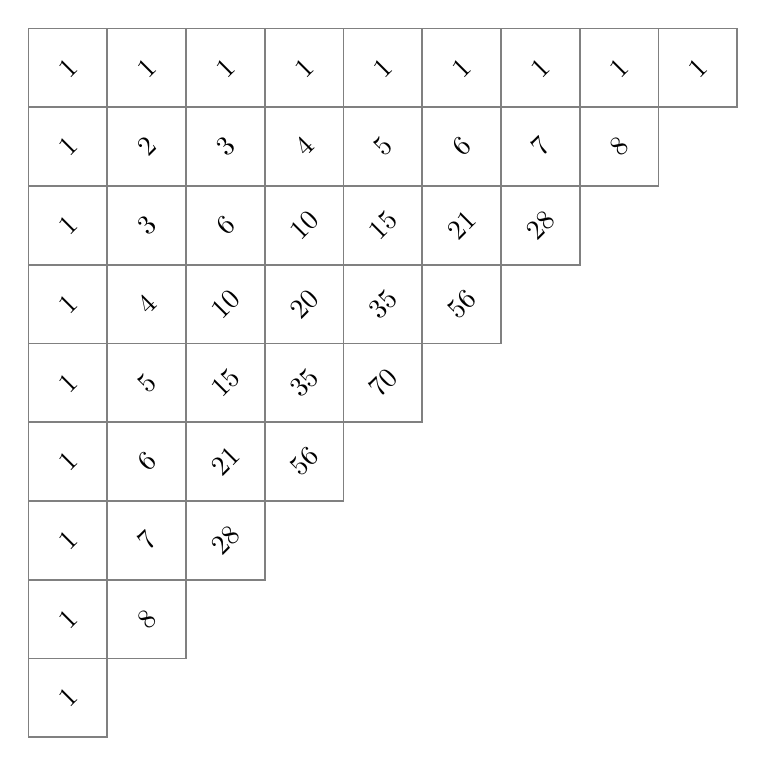
\begin{tikzpicture}[cell/.style = {rectangle,draw=gray,semithick,minimum size=1cm,outer sep=0mm}]
\foreach \i [count=\j from 0] in {1, 1, 1, 1, 1,  1, 1, 1, 1}
    \node[cell] at (\j,  0) {\rotatebox{45}{$\i$}};
\foreach \i [count=\j from 0] in {1, 2, 3, 4, 5,  6, 7, 8}
    \node[cell] at (\j, -1) {\rotatebox{45}{$\i$}};
\foreach \i [count=\j from 0] in {1, 3, 6, 10,15,21,28}
    \node[cell] at (\j, -2) {\rotatebox{45}{$\i$}};
\foreach \i [count=\j from 0] in {1, 4, 10,20,35,56}
    \node[cell] at (\j, -3) {\rotatebox{45}{$\i$}};
\foreach \i [count=\j from 0] in {1, 5, 15,35,70}
    \node[cell] at (\j, -4) {\rotatebox{45}{$\i$}};
\foreach \i [count=\j from 0] in {1, 6, 21,56}
    \node[cell] at (\j, -5) {\rotatebox{45}{$\i$}};
\foreach \i [count=\j from 0] in {1, 7, 28}
    \node[cell] at (\j, -6) {\rotatebox{45}{$\i$}};
\foreach \i [count=\j from 0] in {1, 8}
    \node[cell] at (\j, -7) {\rotatebox{45}{$\i$}};
\foreach \i [count=\j from 0] in {1}
    \node[cell] at (\j, -8) {\rotatebox{45}{$\i$}};
\end{tikzpicture}
}
}
\end{center}
\end{frame}

\begin{frame}[fragile]{}{}
線形再帰ならループと再帰の記述の手間は同じ(実行時間も同じ)。
問題は線形でない場合:スタックを使って自分で機械語実行過程のシミュレーションを書けるならOK。
\end{frame}

\end{document}
